\documentclass{article}
\usepackage[utf8]{inputenc}
\usepackage[top=1in, bottom=1in, left=1in, right=1in]{geometry}
% \usepackage{indentfirst}
\usepackage{amsmath}
\usepackage{amssymb}
\usepackage{graphicx}
    \DeclareGraphicsExtensions{.png, .jpeg}
\usepackage{caption}


\newcommand*{\doublebar}[1]{\overline{\overline{#1}}}
\newcommand*{\unknown}[0]{\;?\;}


\title{MATH 786: Cooperative Game Theory \\ HW01}
\author{Terence Henriod}
\date{\today}

\begin{document}

\maketitle

\begin{abstract}
Linear Programming, Super-Additivity, Convex Games
\end{abstract}


\newpage
\begin{enumerate}
\item Consider the Linear Program $LP$: $z = \max 2x_{1} + 5x_{2}$ \\
    subject to:
    \begin{align}
     x_{1}  +   x_{2}  \le& \; 10 \\
    3x_{1}  +  2x_{2}  \le& \; 24 \\
     x_{1}  +  3x_{2}  \le& \; 24 \\
     x_{1}  ,   x_{2}  \ge& \;  0 \notag
    \end{align}

    \begin{enumerate}
    %
    \item The set of all points satisfying (1), (2), (3) and the the nonnegativity constraints is called the \emph{feasible region} of $LP$. Graph the feasible region of $LP$.
    \textit{Solution}:
    \begin{figure}[h!]
      \centering
      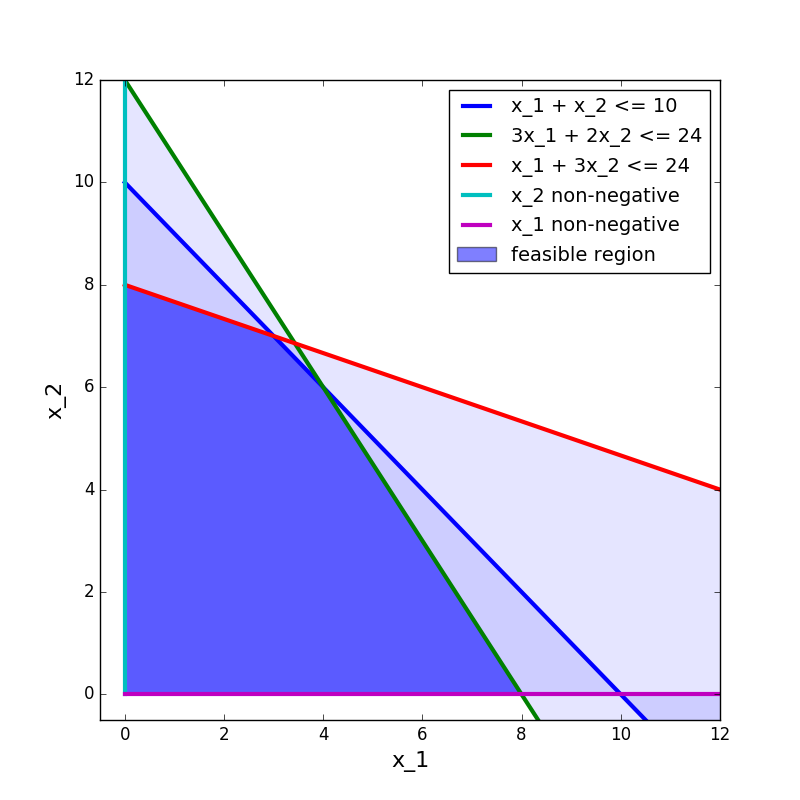
\includegraphics[width=.5\linewidth]{01_a}
      \label{fig:01_a}
    \end{figure}

    %
    \item An \emph{extreme point} of a set $C$ is a point $x$ for which, $y \in C$, $z \in C$, $x = 0.5y + 0.5z \implies y = z = x$. List all of the extreme points of the feasible region of $LP$. \\\\
    \textit{Solution}:\\
    We can find the extreme points by finding the intersections of the lines that define the inequalities.\\
    (Note: each of the equations have been re-arranged to be equal to zero for some of the steps)\\

    Extreme Points: $\mathbf{(4, 6), (3, 7), (0, 8), (8, 0)}$ \\

    Solving for 1 and 2:
    \begin{align*}
    -2(x_{1} + x_{2} - 10)  &=  3x_{1} + 2x_{2} - 24 \\
                      x_{1} &= 4
    \end{align*}
    \begin{align*}
    (4) + x_{2} &= 10 \\
          x_{2} &= 6
    \end{align*}
    Extreme Point 1 $= (4, 6)$ \\

    Solving for 1 and 3:\\
    \begin{align*}
    -1( x_{1} + x_{2} - 10)  &=  x_{1} + 3x_{2} - 24  \\
                     2x_{2}  &=  14  \\
                      x_{2}  &=  7
    \end{align*}
    \begin{align*}
    x_{1} + (7) &= 10 \\
    x_{1}       &= 3
    \end{align*}
    Extreme Point 2 $= (3, 7)$ \\

    Solving for 2 and 3:\\
    \begin{align*}
    3x_{1} + 2x_{2} - 24  &=  -3( x_{1} + 3x_{2} - 24) \\
                 -7x_{2}  &=  -48  \\
                   x_{2}  &=  \frac{48}{7}
    \end{align*}
    \begin{align*}
    x_{1} + 3(\frac{48}{7})  &=  24 \\
    x_{1} + \frac{144}{7}    &=  \frac{168}{7} \\
    x_{1}                    &=  \frac{24}{7}
    \end{align*}
    (Not feasible) Extreme Point 3 $= (\frac{24}{7}, \frac{48}{7})$ \\

    Solving for 3 and constraint $x_1 \ge 0$:\\
    \begin{align*}
    x_{1} + 3x_{2} - 24  &=  -1(x_{1} - 0) \\
            3x_{2} - 24  &=  0 \\
                 3x_{2}  &=  24 \\
                  x_{2}  &=  8 \\
    \end{align*}
    \begin{align*}
    x_{1}  &=  0 \\
    \end{align*}
    Extreme Point 4 $= (0, 8)$ \\

    Solving for 2 and constraint $x_2 \ge 0$:\\
    \begin{align*}
    3x_{1} + 2x_{2} - 24  &=  -2(x_{2} - 0) \\
             3x_{1} - 24  &=  0 \\
                  3x_{1}  &=  24 \\
                   x_{1}  &=  8 \\
    \end{align*}
    \begin{align*}
    x_{2}  &=  0 \\
    \end{align*}
    Extreme Point 5 $= (8, 0)$ \\

    %
    \item Give the dual linear program to $LP$. \\\\
    \textit{Solution}:\\
    To make things easy, I will put the program in matrix form, where

    \[
    c = \begin{bmatrix}
    2 \\
    5
    \end{bmatrix}, \quad
    A = \begin{bmatrix}
    1  &  1 \\
    3  &  2 \\
    1  &  3
    \end{bmatrix}, \quad
    b = \begin{bmatrix}
    10 \\
    24 \\
    24
    \end{bmatrix}, \quad
    x = \begin{bmatrix}
    x_{1} \\
    x_{2}
    \end{bmatrix}
    \]

    If our primal program is 
    $$\max c^{T}x \quad \text{s.t.} \quad Ax \le b, \; x \ge 0$$
    then the dual program will take the form 
    $$\min y^{T}b \quad \text{s.t.} \quad y^{T}A \ge c, \; y \ge 0.$$
    Thus, the dual of the program, $D$, is:

    $D$: $z = \min 10y_{1} + 24y_{2} + 24y_{3}$ \\
    subject to:
    \begin{align}
    y_{1}  +  3y_{2}  +   y_{3}  \ge& \; 2 \\
    y_{1}  +  2y_{2}  +  3y_{3}  \ge& \; 5 \\
    y_{1}  ,   y_{2}  ,   y_{3}  \ge& \; 0 \notag
    \end{align}

    %
    \item Find $z$. HINT: The linear program must solve at one of its extreme points. \\\\
    \textit{Solution}:\\
    Recall that the extreme points are 
    $(4, 6), (3, 7), (0, 8), (8, 0)$ and that we are maximizing $z = \max 2x_{1} + 5x_{2}$. So we have:
    \begin{align*}
    z =            2(2) +            5(6) &=            34  \;             \\
    z =            2(3) +            5(7) &=            41  \; \circledast \\
    z = 2(0)            + 5(8)            &= 40             \;             \\
    z = 2(8)            + 5(0)            &= 40             \;             \\
    \end{align*}
    So $z = 41$

    \end{enumerate}

%
\hfill\newline
\item Suppose $G = (N, V)$, where $N = \{ 1, 2, 3 \}$ and $V$ is given by $V(\emptyset) = 0$, $V(\overline{1}) = 2$, $V(\overline{2}) = 4$, $V(\overline{3}) = 0$, $V(\overline{1, 2}) = 8$, $V(\overline{1, 3}) = 3$, $V(\overline{2, 3}) = 8$, and $V(\overline{1, 2, 3}) = 10$.
    \begin{enumerate}
    %
    \item Is this game superadditive? Give an argument in favor or a counterargument against. \\\\
    \textit{Solution}:\\
    The game is superadditive. For all of the coalitions, none of their ``sub-coalitions" have a greater value.\\
    (Note: I only show work for coalitions whose subsets are proper)
    \begin{align*}
    V(\overline{1, 2}) &\ge V(\overline{1}) + V(\overline{2})                       \rightarrow  8 \ge 2 + 4       \rightarrow  \mathbf{8 \ge 6}   \\
    V(\overline{1, 3}) &\ge V(\overline{1}) + V(\overline{3})                       \rightarrow  3 \ge 2 + 0       \rightarrow  \mathbf{3 \ge 2}   \\
    V(\overline{2, 3}) &\ge V(\overline{2}) + V(\overline{3})                       \rightarrow  8 \ge 4 + 0       \rightarrow  \mathbf{8 \ge 4}   \\
    V(\overline{1, 2, 3}) &\ge V(\overline{1}) + V(\overline{2}) + V(\overline{3})  \rightarrow  10 \ge 2 + 4 + 0  \rightarrow  \mathbf{10 \ge 6}  \\
    V(\overline{1, 2, 3}) &\ge V(\overline{1, 2}) + V(\overline{3})                 \rightarrow  10 \ge 8 + 0      \rightarrow  \mathbf{10 \ge 8}  \\
    V(\overline{1, 2, 3}) &\ge V(\overline{1, 3}) + V(\overline{2})                 \rightarrow  10 \ge 3 + 4      \rightarrow  \mathbf{10 \ge 7}  \\
    V(\overline{1, 2, 3}) &\ge V(\overline{2, 3}) + V(\overline{1})                 \rightarrow  10 \ge 8 + 2      \rightarrow  \mathbf{10 \ge 10} \\
    \end{align*}

    %
    \item Give the 0-normalization for this game. \\\\
    \textit{Solution}:\\
    The 0-normalization of a game is computed by subracting the values of the singleton players from the value of any coalition containing the player. \\
    \begin{align*}
    \bar{V}(\emptyset)           &=  0                                                                                                             \\
    \bar{V}(\overline{1, 2})     &=  V(\overline{1, 2}) - (V(\overline{1}) + V(\overline{2})) = (8) - ((2) + (4)) = 2                              \\
    \bar{V}(\overline{1})        &=  V(\overline{1}) - V(\overline{1}) = (2) - (2) = 0                                                             \\
    \bar{V}(\overline{1, 3})     &=  V(\overline{1, 3}) - (V(\overline{1}) + V(\overline{3})) = (3) - ((2) + (0)) = 1                              \\
    \bar{V}(\overline{2})        &=  V(\overline{2}) - V(\overline{2}) = (4) - (4) = 0                                                             \\
    \bar{V}(\overline{2, 3})     &=  V(\overline{2, 3}) - (V(\overline{2}) + V(\overline{3})) = (8) - ((4) + (0)) = 4                              \\
    \bar{V}(\overline{3})        &=  V(\overline{3}) - V(\overline{3}) = (0) - (0) = 0                                                             \\
    \bar{V}(\overline{1, 2, 3})  &=  V(\overline{1, 2, 3}) - (V(\overline{1}) + V(\overline{2}) + V(\overline{3})) = (10) - ((2) + (4) + (0)) = 4  \\
    \end{align*}

    %
    \item Give the 0-1 normalization for the game. \\\\
    \textit{Solution}:\\
    The 0-1 normalization of a game is computed by of all 0-normalized coalitions by the value of the 0-normalized grand coalition in order for all values to be in the range $[0, 1]$ (assuming the grand coalition has the highest worth). \\
    \begin{align*}
    \bar{\bar{V}}(\emptyset)           &=  0                                                                                          \\
    \bar{\bar{V}}(\overline{1, 2})     &=  \bar{V}(\overline{1, 2}) \div \bar{V}(\overline{1, 2, 3}) = (2) \div (4)    = \frac{2}{4}  \\
    \bar{\bar{V}}(\overline{1})        &=  \bar{V}(\overline{1}) \div \bar{V}(\overline{1, 2, 3})= (0) \div (4)        = 0            \\
    \bar{\bar{V}}(\overline{1, 3})     &=  \bar{V}(\overline{1, 3}) \div \bar{V}(\overline{1, 2, 3}) = (1) \div (4)    = \frac{1}{4}  \\
    \bar{\bar{V}}(\overline{2})        &=  \bar{V}(\overline{1}) \div \bar{V}(\overline{1, 2, 3})= (0) \div (4)        = 0            \\
    \bar{\bar{V}}(\overline{2, 3})     &=  \bar{V}(\overline{2, 3}) \div \bar{V}(\overline{1, 2, 3}) = (4) \div (4)    = 1            \\
    \bar{\bar{V}}(\overline{3})        &=  \bar{V}(\overline{1}) \div \bar{V}(\overline{1, 2, 3})= (0) \div (4)        = 0            \\
    \bar{\bar{V}}(\overline{1, 2, 3})  &=  \bar{V}(\overline{1, 2, 3}) \div \bar{V}(\overline{1, 2, 3}) = (4) \div (4) = 1            \\
    \end{align*}

    %
    \item Graph the core for the game, its 0-normalization, and its 0-1 normalization. Compare and conclude. \\\\
    \textit{Solution}:\\
    The graphs all feature a core (``solution region") of the same shape. After applying either type of normalization, the shapes of the normalized graphs become similar. In all cases, the graphs represent the same information, in that the solution has not truly changed, only been shifted or scaled.

    \begin{figure}[h!]
      \centering
      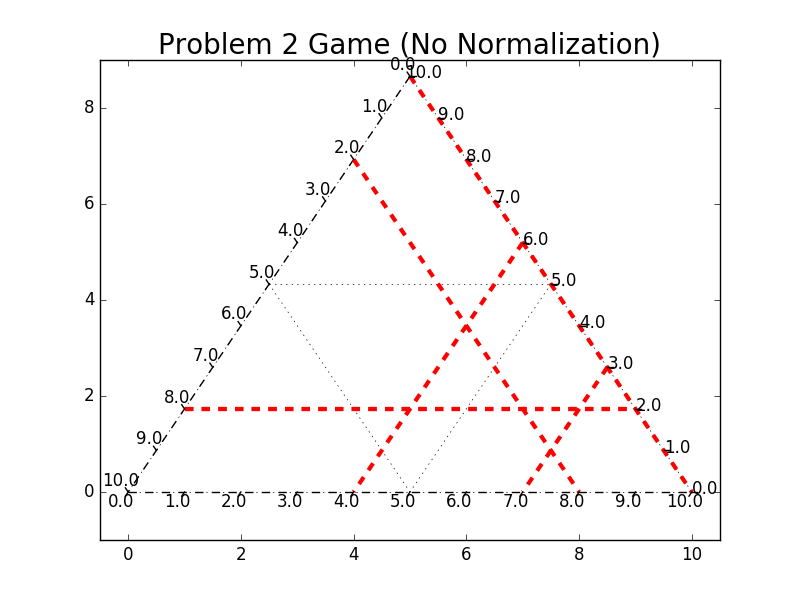
\includegraphics[width=.4\linewidth]{02_c_original}
      \label{fig:02_c_original}
    \end{figure}
    
    \begin{figure}[h!]
    \centering
    \begin{minipage}{.5\textwidth}
      \centering
      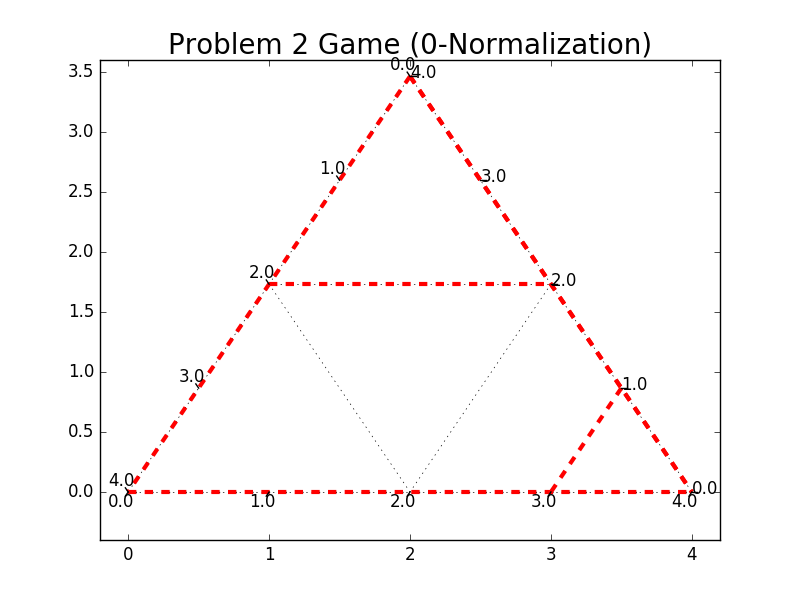
\includegraphics[width=.7\linewidth]{02_c_0norm}
      \label{fig:02_c_0norm}
    \end{minipage}%
    \begin{minipage}{.5\textwidth}
      \centering
      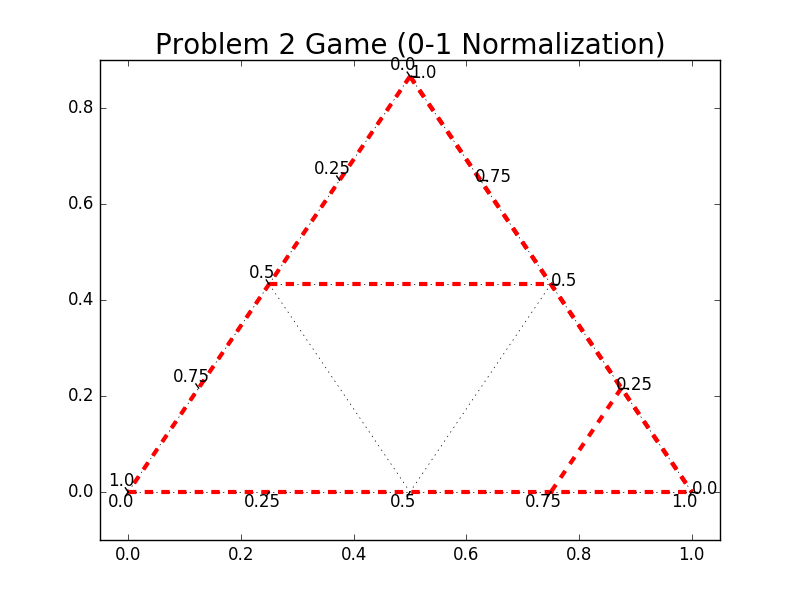
\includegraphics[width=.7\linewidth]{02_c_01norm}
      \label{fig:02_c_01norm}
    \end{minipage}
  \end{figure}

    % Figure generating code
    % # This file is part of inequalities.
    % #
    % # inequalities is free software: you can redistribute it and/or modify
    % # it under the terms of the GNU General Public License as published by
    % # the Free Software Foundation, either version 3 of the License, or
    % # (at your option) any later version.
    % #  
    % # inequalities is distributed in the hope that it will be useful,
    % # but WITHOUT ANY WARRANTY; without even the implied warranty of
    % # MERCHANTABILITY or FITNESS FOR A PARTICULAR PURPOSE.  See the
    % # GNU General Public License for more details.
    % #  
    % # You should have received a copy of the GNU General Public License
    % # along with inequalities.  If not, see <http://www.gnu.org/licenses/>.

    % # This file is part of inequalities.
    % #
    % # inequalities is free software: you can redistribute it and/or modify
    % # it under the terms of the GNU General Public License as published by
    % # the Free Software Foundation, either version 3 of the License, or
    % # (at your option) any later version.
    % #
    % # inequalities is distributed in the hope that it will be useful,
    % # but WITHOUT ANY WARRANTY; without even the implied warranty of
    % # MERCHANTABILITY or FITNESS FOR A PARTICULAR PURPOSE.  See the
    % # GNU General Public License for more details.
    % #
    % # You should have received a copy of the GNU General Public License
    % # along with inequalities.  If not, see <http://www.gnu.org/licenses/>.

    % import ternary

    % FONT_SIZE = 20
    % LINE_ARGS = {'linewidth': 3.0, 'linestyle': '--', 'color': 'red'}

    % #
    % # Original
    % #
    % scale = 10
    % figure, tax = ternary.figure(scale=scale)

    % # Draw Boundary and Gridlines
    % tax.boundary(linewidth=1.0, linestyle='--')
    % tax.gridlines(color="black", multiple=scale / 2)

    % # Set Axis labels and Title
    % tax.set_title("Problem 2 Game (No Normalization)", fontsize=FONT_SIZE)


    % tax.left_parallel_line(2, **LINE_ARGS)
    % tax.right_parallel_line(4, **LINE_ARGS)
    % tax.horizontal_line(0, **LINE_ARGS)
    % tax.horizontal_line(2, **LINE_ARGS)
    % tax.right_parallel_line(7, **LINE_ARGS)
    % tax.left_parallel_line(2, **LINE_ARGS)

    % tax.ticks(axis='lbr', multiple=1.0, linewidth=1.0)

    % tax.show()

    % #
    % # 0-Normalized
    % #
    % scale = 4
    % figure, tax = ternary.figure(scale=scale)

    % # Draw Boundary and Gridlines
    % tax.boundary(linewidth=1.0, linestyle='--')
    % tax.gridlines(color="black", multiple=scale / 2)

    % # Set Axis labels and Title
    % tax.set_title("Problem 2 Game (0-Normalization)", fontsize=FONT_SIZE)

    % tax.horizontal_line(0, **LINE_ARGS)
    % tax.right_parallel_line(0, **LINE_ARGS)
    % tax.left_parallel_line(0, **LINE_ARGS)
    % tax.left_parallel_line(2, **LINE_ARGS)
    % tax.right_parallel_line(3, **LINE_ARGS)
    % tax.horizontal_line(0, **LINE_ARGS)

    % tax.ticks(axis='lbr', multiple=1.0, linewidth=1.0)

    % tax.show()

    % #
    % # 0-1 Normalized
    % #
    % scale = 1
    % figure, tax = ternary.figure(scale=scale)

    % # Draw Boundary and Gridlines
    % tax.boundary(linewidth=1.0, linestyle='--')
    % tax.gridlines(color="black", multiple=scale / 2)

    % # Set Axis labels and Title
    % tax.set_title("Problem 2 Game (0-1 Normalization)", fontsize=FONT_SIZE)

    % tax.horizontal_line(0, **LINE_ARGS)
    % tax.right_parallel_line(0, **LINE_ARGS)
    % tax.left_parallel_line(0, **LINE_ARGS)
    % tax.left_parallel_line(2 / 4, **LINE_ARGS)
    % tax.right_parallel_line(3 / 4, **LINE_ARGS)
    % tax.horizontal_line(0, **LINE_ARGS)

    % tax.ticks(axis='lbr', multiple=0.25, linewidth=1.0)

    % tax.show()
    \end{enumerate}

%
\hfill\newline
\item Suppose $G = (N, V)$, where $N = {A, B, a, b}$ and $V$ is given by $V(\overline{A, a}) = 3$, $V(\overline{B, a}) = 4$, $V(\overline{B, b}) = 2$, $V(\overline{A, a, b}) = 3$, $V(\overline{A, a, B}) = 4$, $V(\overline{A, B, b}) = 2$, $V(\overline{B, a, b}) = 4$, $V(\overline{A, B, a, b}) = 5$, and $V(S) = 0$ for all other coalitions $S$.
    \begin{enumerate}
    %
    \item Find the set of essential coalitions for this game.\\\\
    \textit{Solution}:\\
    Essential coalitions are coalitions whose value is strictly greater than the combined value of any of their possible ``sub-coalitions." Note: I only consider coalitions that can be broken into smaller coalitions (not counting the empty set). \\

    Essential Coalitions: $\overline{A, a}$, $\overline{B, a}$, $\overline{B, b}$, $\overline{A, a}$

    \begin{align*}
    V(\overline{A, B}) &\rightarrow V(\overline{A}), V(\overline{B}) \\
    0                  &\unknown    0              + 0 \\
    0                  &\not>       0                  \implies \text{non-essential} \\
    \end{align*}
    \begin{align*}
    V(\overline{A, a}) &\rightarrow V(\overline{A}), V(\overline{a}) \\
    3                  &\unknown    0              + 0 \\
    3                  &>           0                  \implies \text{essential} \\
    \end{align*}
    \begin{align*}
    V(\overline{A, b}) &\rightarrow V(\overline{A}), V(\overline{b}) \\
    0                  &\unknown    0              + 0 \\
    0                  &\not>       0                  \implies \text{non-essential} \\
    \end{align*}
    \begin{align*}
    V(\overline{B, a}) &\rightarrow V(\overline{B}), V(\overline{a}) \\
    4                  &\unknown    0              + 0 \\
    4                  &>           0                  \implies \text{essential} \\
    \end{align*}
    \begin{align*}
    V(\overline{B, b}) &\rightarrow V(\overline{B}), V(\overline{b}) \\
    2                  &\unknown    0              + 0 \\
    2                  &>           0                  \implies \text{essential} \\
    \end{align*}
    \begin{align*}
    V(\overline{a, b}) &\rightarrow V(\overline{a}), V(\overline{b}) \\
    0                  &\unknown    0              + 0 \\
    0                  &\not>       0                  \implies \text{non-essential} \\
    \end{align*}
    \begin{align*}
    V(\overline{A, B, a}) &\rightarrow V(\overline{A}), V(\overline{B}), V(\overline{a}) \\
    4                     &\unknown    0              + 0              + 0 \\
    4                     &>           0                                   \\
                          &\rightarrow V(\overline{A, B}), V(\overline{a}) \\
    4                     &\unknown    0              + 0                  \\
    4                     &>           0                                   \\
                          &\rightarrow V(\overline{A, a}), V(\overline{B}) \\
    4                     &\unknown    3              + 0                  \\
    4                     &>           3                                   \\
                          &\rightarrow V(\overline{B, a}), V(\overline{A}) \\
    4                     &\unknown    4              + 0                  \\
    4                     &\not>       4                                   \implies \text{non-essential} \\
    \end{align*}
    \begin{align*}
    V(\overline{A, B, b}) &\rightarrow V(\overline{A}), V(\overline{B}), V(\overline{a}) \\
    2                     &\unknown    0              + 0              + 0 \\
    2                     &>           0                                   \\
                          &\rightarrow V(\overline{A, B}), V(\overline{b}) \\
    2                     &\unknown    0              + 0                  \\
    2                     &>           0                                   \\
                          &\rightarrow V(\overline{A, b}), V(\overline{B}) \\
    2                     &\unknown    0              + 0                  \\
    2                     &>           0                                   \\
                          &\rightarrow V(\overline{B, b}), V(\overline{A}) \\
    2                     &\unknown    2              + 0                  \\
    2                     &not>        2                                   \implies \text{non-essential} \\
    \end{align*}
    \begin{align*}
    V(\overline{A, a, b}) &\rightarrow V(\overline{A}), V(\overline{a}), V(\overline{b}) \\
    3                     &\unknown    0              + 0              + 0 \\
    3                     &>           0                                   \\
                          &\rightarrow V(\overline{A, a}), V(\overline{b}) \\
    3                     &\unknown    3              + 0                  \\
    3                     &\not>       3                                   \implies \text{non-essential} \\
    \end{align*}
    \begin{align*}
    V(\overline{B, a, b}) &\rightarrow V(\overline{B}), V(\overline{a}), V(\overline{b}) \\
    4                     &\unknown    0              + 0              + 0 \\
    4                     &>           0                                   \\
                          &\rightarrow V(\overline{B, a}), V(\overline{b}) \\
    4                     &\unknown    4              + 0                  \\
    4                     &\not>       4                                   \implies \text{non-essential} \\
    \end{align*}
    \begin{align*}
    V(\overline{A, B, a, b}) &\rightarrow V(\overline{A}), V(\overline{B}), V(\overline{a}), V(\overline{b}) \\
    5                        &\unknown    0              + 0              + 0              + 0 \\
    5                        &>           0                                   \\
                             &\rightarrow V(\overline{A, B}), V(\overline{a}), V(\overline{b}) \\
    5                        &\unknown    0                 + 0              + 0               \\
    5                        &>           0                                                    \\
                             &\rightarrow V(\overline{A, a}), V(\overline{B}), V(\overline{b}) \\
    5                        &\unknown    3                 + 0              + 0               \\
    5                        &>           3                                                    \\
                             &\rightarrow V(\overline{A, b}), V(\overline{B}), V(\overline{a}) \\
    5                        &\unknown    0                 + 0              + 0               \\
    5                        &>           0                                                    \\
                             &\rightarrow V(\overline{B, a}), V(\overline{A}), V(\overline{b}) \\
    5                        &\unknown    4                 + 0              + 0               \\
    5                        &>           4                                                    \\
                             &\rightarrow V(\overline{B, b}), V(\overline{A}), V(\overline{a}) \\
    5                        &\unknown    2                 + 0              + 0               \\
    5                        &>           2                                                    \\
                             &\rightarrow V(\overline{a, b}), V(\overline{A}), V(\overline{B}) \\
    5                        &\unknown    0                 + 0              + 0               \\
    5                        &>           0                                                    \\
                             &\rightarrow V(\overline{A, B}), V(\overline{a, b}                \\
    5                        &\unknown    0                 + 0                                \\
    5                        &>           0                                                    \\
                             &\rightarrow V(\overline{A, a}), V(\overline{B, b}                \\
    5                        &\unknown    3                 + 2                                \\
    5                        &\not>       5                                                    \implies \text{non-essential} \\
    \end{align*}

    %
    \item Find a core vector for this game. \\\\
    \textit{Solution}:\\
    Given that the core of a game must satisfy:
    \begin{align}
    \sum^{n}_{i = 1}{x_{i}}  &=    V(N)                                &  \text{efficiency}\\
    \sum_{i \in S}{x_{i}}    &\ge  V(S) \text{\; for \;} S \in 2^{N}   &  \text{stability}
    \end{align}
    Consider the payoff vector $\vec{x} = (A: 0, B: 2, a: 3, b: 0)$ (admittedly, I found this vector through trial and error as opposed to a more formal method). It satisfies the efficiency condition because $\sum_{x_{i} \in \vec{x}}{x_{i}} = V(N) = 5$.
    The stability condition also holds:
    (Note: I do not consider the constraints where the sum need only be $\ge 0$ since the constraint is clearly met using non-negative payoffs for each player)
    \begin{align*}
    S = \overline{A, a}     &\rightarrow 1(0) + 0(2) + 1(3) + 0(0) \ge 3  \implies  3  \ge  3\\
    S = \overline{B, a}     &\rightarrow 0(0) + 1(2) + 1(3) + 0(0) \ge 4  \implies  5  \ge  4\\
    S = \overline{B, b}     &\rightarrow 0(0) + 1(2) + 0(3) + b(0) \ge 2  \implies  2  \ge  2\\
    S = \overline{A, B, a}  &\rightarrow 1(0) + 1(2) + 1(3) + 0(0) \ge 4  \implies  5  \ge  4\\
    S = \overline{A, B, b}  &\rightarrow 1(0) + 1(2) + 0(3) + 1(0) \ge 2  \implies  2  \ge  2\\
    S = \overline{A, a, b}  &\rightarrow 1(0) + 0(2) + 1(3) + 1(0) \ge 3  \implies  3  \ge  3\\
    S = \overline{B, a, b}  &\rightarrow 0(0) + 1(2) + 1(3) + 1(0) \ge 4  \implies  5  \ge  4\\
    \end{align*}

    %
    \item Is this game convex? Give an argument in favor or else a counterexample against. \\\\
    \textit{Solution}:\\
    The game is not convex. Recall that a game is convex if $V(S_{1}) + V(S_{2}) \le V(S_{1} \cup S_{2}) + V(S_{1} \cap S_{2})$ for all $S_{1}, S_{2}$ in $2^{N}$.
    Consider the coalitions $S_{1} = \overline{ABa}$ and $S_{2} = \overline{ABb}$. Applying the convexity condition, we have:
    \begin{align*}
    V(\overline{ABa}) + V(\overline{ABb})  &\le      V(\overline{ABa} \cup \overline{ABb})      + \overline{ABa} \cap \overline{ABb}) \\
    4                 + 2                  &\le      V(\overline{A, B, a, b})                   + V(\overline{A, B}) \\
    6                                      &\le      5                                          + 0 \\
    6                                      &\not\le  5 \\
    \end{align*}
    Since the condition does not hold for all $S_{1}$, $S_{2}$ in $2^{N}$, the game cannot be convex.

    \end{enumerate}

%
\hfill\newline
\item Let $G = (N, V)$, where $N = \{1, \dots, n\}$ and $V(S) = |S|^{2}$ for all $S$ in $2^{N}$. Show that $G$ is a convex game. \\\\
\textit{Solution}:\\
Recall that a game is convex if $V(S_{1}) + V(S_{2}) \le V(S_{1} \cup S_{2}) + V(S_{1} \cap S_{2})$ for all $S_{1}, S_{2}$ in $2^{N}$. For $G$ to be convex, this condtion, call it $\circledast$, must hold true.

Let $a = |S_{1}|$, $b = |S_{2}|$, $k = a + b$, and $c = |S_{1} \cup S_{2}|$, which leads to $k - c =  |S_{1} \cap S_{2}|$, \, $a, b \le c$, \, and $k - c \le a, b$.

When comparing $S_{1}s$ and $S_{2}s$, we can consider how each unique pair is related to another by one player that can change either the size of the union of the coalitions or the size of the intersection of the coalitions. By considering all such pairs and relations, we will end up considering all possible pairs $S_{1}s$ and $S_{2}s$. It is not possible for one player to affect both the union and the intersection at the same time. It is not possible to increase the size of the union and the intersection simultaneously by adding a single player to one coalition since in order to increase the size of the union, a player must not be present in either coalition, but in order to increase the size of the intersect, the player must have already been in one of the coalitions, and this is a contradiction. The converse is true for removing a player as well.

I will now use two inductive proofs to show that $\circledast$ holds for $G$, and thus $G$ is a convex game.

First, consider the increase on each side of the inequality of $\circledast$ when adding a player a player that was not in either coalition originally to one of the coalitions (increasing only the size of their union, but not intersection).

For a base case, let $a = b = 0$. Then we have $0^{2} + 0^{2} \le 0^{2} + 0^{2} \implies 0 \le 0$. The base case holds.

Now assume that for some pair of $S_{1}$ and $S_{2}$, $circledast$ is satisfied.

To show that for the next pair of $S_{1}$ and $S_{2}$ where we have added a player that increases the size of the union, call it $S_{1}^{\prime}$ and $S_{2}$, we consider the increases on both sides of the inequality.
For the left hand side we have:
\begin{align*}
lhs-increase  &=  ((a + 1)^{2} + b^{2})    - (a^{2} + b^{2})  \\
              &=  (a^{2} + b^{2} + 2a + 1) - (a^{2} + b^{2})  \\
              &=  2a + 1
\end{align*}
For the right hand side we have:
\begin{align*}
rhs-increase  &=  ((c + 1)^{2} + (k - c)^{2}) - (c^{2} + (k - c)^{2})  \\
              &=  (c + 1)^{2}  - c^{2} \\
              &=  c^{2} + 2c + 1 - c^{2} \\
              &=  2c + 1 \\
\end{align*}
This gives:
\begin{align*}
2a + 1 &\le 2c + 1 \\
a      &\le c + 1 \\
\end{align*}
Which is true because even $a \le c$ is true by the definitions set earlier. Thus, if $\circledast$ holds for some $S_{1}$ and $S_{2}$, it will hold for the corresponding $S_{1}^{\prime}$ and $S_{2}$. So, by induction, I have shown that $\circledast$ holds for $G$ for all $S_{1}s$ and $S_{2}s$ that are related by a player that affects the size of the union of the sets, with $a, b \ge 0$.

Now, consider the decrease on each side of the inequality of $\circledast$ when removing a player a player that was in both coalitions originally from one of the coalitions (decreasing only the size of their intersection, but not their union).

For a base case, let $a = b = k - c$, with $a, b > 0$. Then we have
\begin{align*}
a^{2} + b^{2}  &\le  c^{2} + (k - c)^{2} \\
a^{2}          &\le  c^{2} \\
a              &\le  c \\
\end{align*}
 Which is must be true as stated earlier. The (starting) base case holds.
As a (stopping) base case, consider $a = b = 0$ as we did before, which, of course, also holds.

Now assume that for some pair of $S_{1}$ and $S_{2}$, $circledast$ is satisfied.
To show that for the next pair of $S_{1}$ and $S_{2}$ where we have removed a player that decreases the size of the intersection, call it $S_{1}^{\prime}$ and $S_{2}$, we consider the decreases on both sides of the inequality.
For the left hand side we have:
\begin{align*}
lhs-decarease  &=  ((a - 1)^{2} + b^{2})    - (a^{2} + b^{2})  \\
               &=  (a^{2} + b^{2} - 2a + 1) - (a^{2} + b^{2})  \\
               &=  -2a + 1
\end{align*}
For the right hand side we have:
\begin{align*}
rhs-decarease  &=  (c^{2} + (k - c - 1)^{2}) - (c^{2} + (k - c)^{2})  \\
               &=  (k - c - 1)^{2}) - (k - c)^{2} \\
               &=  (a + b - c - 1)^{2}) - (a + b - c)^{2} \\
               &=  (a^{2} + b^{2} + c^{2} + 2ab - 2ac - 2bc - 2a - 2b + 2c + 1) - (a^{2} + b^{2} + c^{2} + 2ab - 2ac - 2bc) \\
               &=  -2a - 2b + 2c + 1 \\
\end{align*}
This gives:
\begin{align*}
-2a + 1 &\ge -2a - 2b + 2c + 1 \\
 0      &\ge 2b - 2c \\
 0      &\ge b - c \\
\end{align*}
Which is true since $b < c$, making the right side negative. This proves that $\circledast$ holds for $G$ for all $S_{1}s$ and $S_{2}s$ that are related by a player that affects the size of the intersection of the sets. Thus, if $\circledast$ holds for some $S_{1}$ and $S_{2}$, it will hold for the corresponding $S_{1}^{\prime}$ and $S_{2}$ down to the case where $a = b = 0$. So, by induction, I have shown that $\circledast$ holds for $G$ for all $S_{1}s$ and $S_{2}s$ that are related by a player that affects the size of the intersection of the sets, with $a, b \le k - c$ and $a, b \ge 0$.

If $\circledast$ holds for both relations, then we have shown that for all possible $S_{1}s$ and $S_{2}s$ that $G$ is convex.

%
\hfill\newline
\item The \emph{glove game} is a TU-game with $n = m + p$ players. Of the players, $m$ are initially endowed with a single left glove, and the other $p$ players are initially endowed with a single right glove. Suppose that singleton gloves are worthless, but that glove pairs (i.e., a left glove and a right glove) are worth \$5.
    \begin{enumerate}
    %
    \item Write down an expression for the characteristic function of this game. HINT: it will help to define the sets $M$ and $P$ as the set of players who initially own a left glove and right glove respectively. \\\\
    \textit{Solution}:\\
    With $M$ and $P$ defined as above, also let $u$ be defined as the number of players in the coalition coming from $M$ and $v$ be the number of players coming from $P$. Then the following function should define the value of any coalition in this game:
    $$ V(S) = 5 * \min u, v $$

    %
    \item Find the core of the game. HINT: there will be two cases, depending upon the relationship between $m$ and $p$. \\\\
    \textit{Solution}:\\
    The two cases are $m = p$ and $m \neq p$. \\
    
    In the first case where $m = p$, there the core consists of three vectors: one where $V(N)$ is distributed evenly across all of the players from $m$ (i.e. each $m$ player gets \$5) and the players from $p$ get \$0, the reverse, where all players from $p$ get \$5 and players from $m$ get \$0, and the third is where the payoff is distributed equally over all of the players. Note though, that the case where $m = p = 1$ is a special case, and the payoff can actually be distributed any way between the two players as long as they receive non-negative amounts. \\

    In the second case, where $m \neq p$, then the core consists of only one vector: $V(N)$ is distributed evenly across all of the players from the smaller of $m$ and $p$, and the players from the larger set get \$0. \\

    In showing that these are the core vectors, for any coalition $S$, I will refer to the players coming from the set of the smaller of $S \cap M$ and $S \cap P$ as the ``minority players", and players from the larger of $S \cap M$ and $S \cap P$ as the ``majority players." Also, recall the definitions of \emph{efficiency} and \emph{stability} (which a vector $\vec{x}$ must satisfy to be in the core):
    \begin{align}
    \sum^{n}_{i = 1}{x_{i}}  &=    V(N)                                &  \text{efficiency}\\
    \sum_{i \in S}{x_{i}}    &\ge  V(S) \text{\; for \;} S \in 2^{N}   &  \text{stability}
    \end{align}

    To show this is true for the first case, consider first the case where payoff is distributed perfectly evenly. Clearly this vector satisfies the core requirements because it is efficient, and for any coalition, the caolition is stable because the payoffs of the players that form pairs will sum to the value of the coalition itself. Assume we can shift \emph{some} (but not \emph{all}) payment away from one player of $M$, call them $a$, to a player of $P$, call them $b$. Now consider a coalition featuring two players, one from $M$ and one from $P$, where the $M$ player is $a$, and the player from $P$ is not $b$. This would violoate stability because the sum of the individual payoffs for the coalition is less than the value of that coalition. This is a contradiction to the assumption, so it must be that we cannot shift payment from $a$. Now consider shifting \emph{all} of the payment from $a$ to $b$. If we were to do this, it is possible to have the 2-player coalition $\overline{a, b}$ that does satisfy stability, but any other 2-player coalition featuring player $a$ and a player from $P$ will violate stability ($0 + 2.5 \not\ge 5$). To avoid this, if we distribute that payoff evenly between only players of one of the sets $M$ or $P$, then we can never have a coalition that will violate stability because any time there is a pair of players present that increase the payoff for the coalition, one of the players will bring the pay that will satisfy the stability condition into the equation. This, of course applies to any game with $n > 2$ since we can just consider the last player of $M$ and the last player of $P$ as the 2-player coalition as long as the rest of the players satisfy the core constraints. In the special case with $m = p = 1$, the payoff can be distributed arbitrarily (as long as each player receives a non-negative payoff) and stability will be satisfied. \\

    To show this is true for the second case, consider the $S \in N$, in particular all $S^{\prime}$ that have at least one pair of gloves in them and also represent coalitions that all share the same number of ``minority players" and exclude at least one ``majority player." Assume it is possible to distribute some of the payoff away from one minority to one majority player, call that majority player $a$, so that all of the other majority players have \$0 and all of the minority players have \$5 (except the one we shifted money away from). In doing so, stability holds for the $S^{\prime}$s that contain $a$, but it is violated for any $S^{\prime}$s that does not contain $a$. This contradicts our assumption, so all of the payoff must reside with the minority players. \\

    By a similar argument, we cannot pay the minority players unevenly. If we were to consider coalitions that exclude at least one minority player, call them $b$, assume that we may distribute payoff away from one other minority player, $c$, to $b$. Again, in any $S^{\prime}$ containing $b$, stability holds, but in any $S^{\prime}$s containing $c$ and not $b$, stability is violated. \\

    In the special cases where $m = 0$ and $p = 1$ and vice versa, there will be no payoff to distribute, so the cores will consist of a zero vector. \\

    \end{enumerate}

%
\hfill\newline
\item For each of the following families of coalitions, determine whether they are (a) balanced; (b) minimal balanced; and/or (c) proper minimal balanced. In all cases, assume $N = \{1, \dots, n\}$.\\\\
\textit{Solution}:\\
Recall that for a family $T$ to be (a) balanced, there must exist \emph{balancing weights} $\{\delta_{S}\}_{S \in T}$ s.t. for every player of the game $i$:
    $$\sum_{S \in T \; \text{s.t.} \; S \ni i}{\delta_{S}} \; = \; 1 \qquad \circledast$$
Note that if some player $i$ is not contained in a family, then there cannot be any balancing weigts that sum to $1$ for that player, thus leaving the family unbalanced (i.e. if $S = \emptyset$, there is nothing to sum over in the expression above).
For a family to be (b) minimal balanced, it must be balanced and no proper sub-family of $T$ can be balanced.
Finally, for a family to be (c) proper minimal balanced, it must be minimal balanced and $S_{1} \cap S_{2} \ne \emptyset$ for all $S_{1}$, $S_{2}$ in $T$ must hold.

    \begin{enumerate}
    %
    \item $n = 5$, $T = \{\overline{1, 2, 3}\,, \; \overline{1, 2, 4}\,, \; \overline{1, 2, 5}\,, \; \overline{1, 3, 4}\,, \; \overline{1, 3, 5}\,, \; \overline{1, 4, 5}\,, \; \overline{2, 3, 4}\,, \; \overline{2, 3, 5}\,, \; \overline{2, 4, 5}\,, \; \overline{3, 4, 5}\}$\\\\
    \textit{Solution}:\\
    \textbf{(a)} \\
    $T$ is (a) balanced, since every player appears in exactly $6$ coalitions, we can balance the family with all $\delta_{S} = \frac{1}{6}$. $T$ is not minimal balanced since the sub-family $T^{\prime} = \{\overline{1, 2, 3}\,, \; \overline{2, 3, 4}\,, \; \overline{3, 4, 5}\,, \; \overline{1, 4, 5}\,, \; \overline{1, 2, 5}\,\}$ can be balanced with all $\delta_{S} = \frac{1}{3}$. Since $T$ is not minimal balanced, it cannot be proper minimal balanced.
    \\

    %
    \item $n = 4$, $T = \{\overline{1, 2}\,, \; \overline{1, 3}\,, \; \overline{2, 3}\}$\\\\
    \textit{Solution}:\\
    $T$ is not balanced in this scenario, and therefore neither minimal balanced not proper minimal balanced, because when we consider $i = 4$, condition $\circledast$ does not hold.
    \\

    %
    \item $n = 6$, $T = \{\overline{1, 2}\,, \; \overline{3, 4, 5}\,, \; \overline{6}\}$\\\\
    \textit{Solution}:\\
    \textbf{(a), (b)}\\
    This family is a partition of $N$. Therefore, it is (a) balanced with all weights $\delta_{S} = 1$. $T$ is (b) minimal balanced, since no sub-family $T^{\prime}$ is balanced because $T^{\prime}$ would not contain all of the players, violating $\circledast$. $T$ is not proper minimal balaced because there is at least one disjoint pair of coalitions in the family (consider $\overline{1, 2} \cap \overline{3, 4, 5} = \emptyset$).
    \\

    %
    \item $n = 8$, $T = \{\overline{1, 2, 3, 4, 5}\,, \; \overline{3, 4, 5, 6, 7, 8}\,, \; \overline{1, 2, 6, 7, 8}\}$\\\\
    \textit{Solution}:\\
    \textbf{(a), (b), (c)}\\
    Each player appears exactly twice in the sets of this family, so this family can be (a) balanced with $\{\delta_{S}\}_{S \in T}$ where all $\delta_{S} = \frac{1}{2}$. $T$ is also (b) minimal balanced because no sub-family can be balanced, any one of the coalitions do not contain the full player set, and any two of the coalitions will feature some of the players twice but others only once - thus being impossible to balance. Finally, $T$ is (c) proper minimal balanced because $\overline{1, 2, 3, 4, 5} \cap \overline{3, 4, 5, 6, 7, 8} \ne \emptyset$, $\overline{1, 2, 3, 4, 5} \cap \overline{1, 2, 6, 7, 8} \ne \emptyset$, and $\overline{3, 4, 5, 6, 7, 8} \cap \overline{1, 2, 6, 7, 8} \ne \emptyset$.

    \end{enumerate}

\end{enumerate}

\end{document}
